\section{Simulation d'événements}\label{chapter-LHC-section-MC}
La simulation d'événements permet de comparer les résultats expérimentaux aux prédictions théoriques.
Elle se déroule en plusieurs étapes.
\par Premièrement, les processus physiques prédits par le modèle théorique à tester sont simulés.
La nature probabiliste des ces processus mène à utiliser un générateur d'événements Monte-Carlo.
Cette étape est détaillée en section~\ref{chapter-LHC-section-MC-subsec-evt_gen}.
Les particules issues des collisions sont alors obtenues ainsi que toute l'historique de leurs formations à partir des particules initiales entrant en collision.
\par Deuxièmement, la propagation de ces particules dans le détecteur, leurs interactions avec ses différents composants et les signaux qui en résultent sont également simulés.
Cette simulation du détecteur est l'objet de la section~\ref{chapter-LHC-section-MC-subsec-detector_sim}.
Cette méthode permet d'obtenir une estimation des signaux devant être observés avec le détecteur si le modèle testé est le modèle décrivant effectivement l'Univers.
\par
La reconstruction des événements telle que décrite dans la section précédente peut alors avoir lieu.
Toutefois, des écarts résiduels existent entre les estimations obtenues par simulation et la réalité.
Des analyses dédiées permettent d'obtenir les corrections à appliquer aux données simulées afin de réduire ces écarts.
\subsection{Génération d'événements}\label{chapter-LHC-section-MC-subsec-evt_gen}
La description analytique de l'interaction entre les constituants des protons lors des collisions est réalisée grâce à la théorie des perturbations.
À l'aide des règles de Feynman présentées dans l'annexe~\refApFmf, il est possible de calculer l'\og élément de matrice \fg{} permettant de décrire le passage d'un état initial à un état final.
Les événements sont alors générés à un ordre perturbatif donné à l'aide de
\MADGRAPH~\cite{madgraph5}
ou
\PYTHIA~\cite{pythia6.4,pythia8.2}
par exemple.
La plupart des processus sont ainsi disponibles à l'ordre dominant (LO, \emph{Leading Order}).
Dans certains cas, les ordres supérieurs (NLO, \emph{Next-to-Leading Order}, NNLO, \emph{Next-to-Next-to-Leading Order}, etc.) sont également disponibles grâce à des générateurs NLO tels que
\POWHEG~\cite{Alioli:2010xd} et
\MCATNLO~\cite{MCATNLO}.
\par Ces générateurs donnent ainsi le processus initial de la collision, duquel sont issues de nouvelles particules.
Cependant, les particules possédant une charge de couleur comme les quarks ne peuvent subsister seules à cause du confinement de couleur, phénomène abordé dans le chapitre~\refChMSSM.
Des étapes de génération supplémentaires sont alors nécessaires afin de décrire l'évolution ultérieure de ces particules.
Il s'agit de la formation de la gerbe partonique et de l'hadronisation, détaillées dans le chapitre~\refChMSSM.
Des générateurs comme
\PYTHIA~\cite{pythia6.4,pythia8.2} et
\HERWIG~\cite{herwig}
permettent de simuler ces étapes ultérieures.
\par Lors d'une collision de protons et plus généralement de hadrons, plusieurs interactions entre les constituants des hadrons peuvent survenir, comme illustré sur la figure~\ref{fig-event_generator_HEP-2-Figure1-1}.
L'interaction emportant la plus grande fraction de l'énergie des hadrons est l'\og interaction dure \fg{}.
Les autres interactions constituent l'événement sous-jacent.
\begin{figure}[h]
\centering
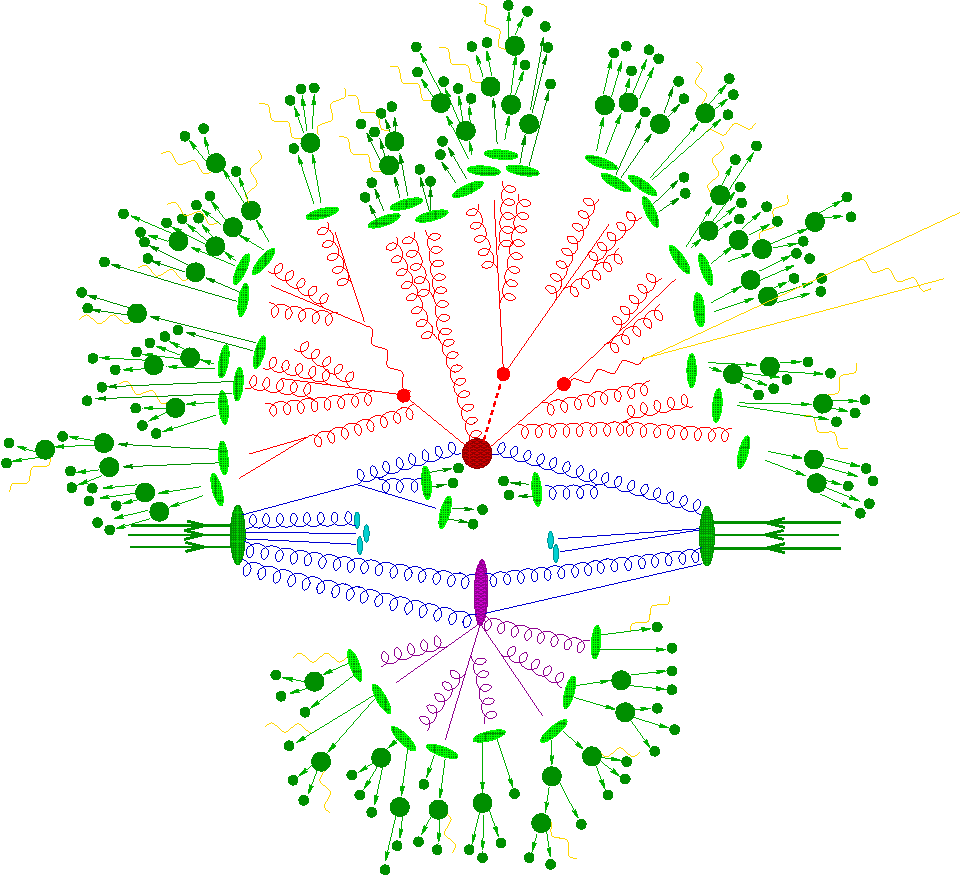
\includegraphics[width=15cm]{\PhDthesisdir/plots_and_images/from_event_generator_HEP/2-Figure1-1.tex}
\caption[Représentation d'une collision de protons.]{Représentation d'une collision de protons~\cite{event_generator_HEP}.}
\label{fig-event_generator_HEP-2-Figure1-1}
\end{figure}
\subsection{Simulation du détecteur}\label{chapter-LHC-section-MC-subsec-detector_sim}
Une fois simulée la physique de l'événement, indépendante du détecteur utilisé, il faut simuler la réponse du détecteur à cet événement.
La propagation des particules est alors simulée en prenant en compte la présence du champ magnétique courbant les trajectoires des particules chargées.
\par Les désintégrations de certaines particules ont lieu dans le volume du détecteur et sont également simulées.
La modélisation du détecteur permet de simuler les déviations des particules dues à la traversée de la matière constituant le détecteur~\cite{moliere_scat_1,moliere_scat_2} ainsi que les interactions propres à la détection de ces particules comme les traces, les gerbes électromagnétiques et hadroniques.
Alors, la modélisation de l'électronique et du système de déclenchement donnent une simulation de la réponse complète du détecteur à l'événement physique généré.
\par Cette simulation du détecteur est basée sur le logiciel
\GEANTfour~\cite{geant4_2003,geant4_2006,geant4_2016}.
La modélisation complète et précise du détecteur (câblage interne, système de refroidissement, éléments de structure, etc.) permet d'obtenir des résultats fidèles à la réalité.
Les signaux simulés du détecteur ainsi obtenus sont alors traités, comme dans le cas des données réelles, par l'algorithme de \emph{Particle Flow}, abordé dans la section précédente, permettant de reconstruire l'événement physique à partir des signaux du détecteur.
\subsection{Corrections apportées aux simulations}
Des écarts résiduels entre les données simulées et la réalité qu'elles doivent décrire existent et sont mesurés par des analysés dédiées.
Ces analyses fournissent alors des corrections à appliquer aux simulations.
Il existe également des données hybrides, dont les événements sont construits à partir de données réelles et simulées.
Il s'agit des données dites \og encapsulées \fg{} (\emph{embedded}) présentées dans le chapitre~\refChHTT, pour lesquelles certaines de ces corrections peuvent être différentes de celles à appliquer aux données \SI{100}{\%} simulées.
\subsubsection{Pondérations dues aux collisions}
\paragraph{Pondération de l'empilement (\emph{Pileup reweighting})}
Les données simulées sont générées avec un réglage donné de luminosité instantanée, relié à la quantité d'empilement obtenu.
Or, la production de ces jeux de données est souvent faite avant la mesure de ces observables dans les données réelles.
Afin de corriger la différence sur le profil d'empilement obtenu, un poids est appliqué aux événements simulés afin que ce profil soit cohérent avec celui des données réelles.
\paragraph{Pondération du \emph{prefiring}}
En 2016 et 2017, le niveau L1 du système de déclenchement de CMS présentait un défaut.
Dans la partie à haute $\eta$ du ECAL, des objets physique responsables du déclenchement du L1 étaient associés à l'événement précédent.
Seul un événement sur trois consécutifs pouvant être enregistré, l'efficacité de la prise de données est moindre qu'attendue.
De plus, cette efficacité dépend de la topologie des événements.
En l'occurrence, les événements avec des jets de hautes valeurs de $\eta$ sont particulièrement touchés par cet effet.
Une pondération est alors appliquée afin de corriger cet effet.
Selon la topologie de l'événement, il peut être de \num{1.0} ou descendre à des valeurs de l'ordre de \num{0.95}.
\subsubsection{Reconstruction et identification des particules individuelles}
\paragraph{Efficacité d'identification et isolation des muons et des électrons (\emph{muon/electron ID/iso efficiency})}
%L'efficacité de l'identification des muons et des électrons ainsi que la mesure de leur isolation peut différer entre données réelles et simulées.
Des facteurs correctifs sont déterminés par le groupe \Higgs\tau\tau.
Ils sont appliqués individuellement à chaque muon et électron utilisé dans les analyses et dépendent de l'année ainsi que de la nature des données, simulées ou encapsulées.
\paragraph{Efficacité du trajectographe (\emph{tracking efficiency})}
L'efficacité de la reconstruction des traces des particules n'est pas la même selon la nature des données, réelles ou simulées, comme l'ont constaté les \POG s EGamma (électrons et photons) et \emph{tracking} dans le cas des électrons et des muons.
%Le cas des muons a une incidence sur les \tauh\ des données encapsulées.
Des facteurs d'échelle, que ces \POG s fournissent, sont appliqués afin de corriger cet effet.
\paragraph{Énergie des électrons (\emph{electron energy scale})}
La mesure de l'énergie des électrons dans les données simulées est corrigée selon les recommandations du \POG\ EGamma~\cite{EGammaPOG}, résumées dans le tableau~\ref{tab-chapter-HTT_analysis-section-corrections-eleES}.
\begin{table}[h]
\centering
\begin{tabular}{lccc}
\toprule
Région du détecteur & 2016 & 2017 & 2018\\
\midrule
\CMSBarrel\ ($\abs{\eta}<\num{1.479}$) & $\num{-0.24}\pm\num{0.5}$ & $\num{-0.07}\pm\num{0.5}$ & $\num{-0.33}\pm\num{0.5}$ \\
\CMSEndcaps\ ($\abs{\eta}>\num{1.479}$) & $\num{-0.70}\pm\num{1.25}$ & $\num{-1.13}\pm\num{1.25}$ & $\num{-0.56}\pm\num{1.25}$ \\
\bottomrule
\end{tabular}
\caption[Corrections à l'énergie des électrons.]{Corrections à l'énergie des électrons en \SI{}{\%} avec incertitude pour les trois années du Run~II.}
\label{tab-chapter-HTT_analysis-section-corrections-eleES}
\end{table}
\subsubsection{Jets}
\paragraph{Énergie des jets (\emph{Jet Energy Calibration})}
La mesure de l'énergie des jets et la résolution sur celle-ci sont corrigées.
Le chapitre~\refChJERC\ est dédié à ces corrections, elle y sont détaillées.
\paragraph{Correction de l'efficacité du \quarkb-\emph{tagging}}
%\subparagraph{\todo{move?} Efficacité du \quarkb-\emph{tagging} (\emph{Btag efficiency})}
Le \POG\ BTV fournit des facteurs correctifs $SF$ à l'efficacité du \quarkb-\emph{tagging} en fonction de la saveur du jet au niveau généré, des propriété cinématiques du jet et du point de fonctionnement du discriminateur de \quarkb-\emph{tagging} utilisé~\cite{BTV}.
Plus de détails sur l'obtention de ces facteurs sont disponibles dans la référence~\cite{Sirunyan_heavy_flavor_jets_2018}.
Le taux de mauvaise identification est également corrigé.
\par
Pour cela, une méthode de promotion-relégation (\emph{promote-demote}) est utilisée.
Une fraction des jets tagués~\quarkb, \ie\ identifiés comme issus d'un quark~\quarkb, est relégué à l'état de jet non tagué~\quarkb\ et
une fraction des jets non tagués~\quarkb\ est promue à l'état de jet tagué~\quarkb.
Un jet peut être promu si son facteur correctif $SF$ est supérieur à 1.
Sinon, il peut être relégué.
La probabilité d'être promu ou relégué s'exprime
\begin{equation}
P(\text{promu}) = \frac{SF-1}{\frac{1}{\epsilon}-1}, SF > 1
\msep
P(\text{relégué}) = 1 - SF, SF < 1
\mend[,]
\end{equation}
avec $\epsilon$ l'efficacité du \quarkb-\emph{tagging}.
\subsubsection{Taus hadroniques}
\paragraph{Efficacité d'identification et isolation des \tauh\ (\emph{\tauh\ ID/iso scale factors})}
L'efficacité d'identification des \tauh\ n'est pas la même dans les données réelles et simulées~\cite{TauPOG}.
Des facteurs correctifs sont déterminés par le \POG\ tau à partir d'événements Drell-Yan dans le canal \mu\tauh, \ie\ lorsqu'un des leptons \tau\ issus du \Zboson\ se désintègre en muon et l'autre en \tauh.
Ils sont de plus donnés séparément pour les données simulées et encapsulées.
De même, la mesure de l'isolation des \tauh\ est ajustée dans les simulations.
\paragraph{Taux de mauvaise identification $\mu\to\tauh$ (\emph{$\mu\to\tauh$ fake rate})}
Il est possible que des muons soient identifiés à tort comme des \tauh.
Il s'agit alors de mauvais \tauh\ ou \og \ftauhs \fg{}.
L'efficacité de la réjection de ces \ftauhs\ diffère entre données réelles et simulées~\cite{TauPOG}.
Un facteur d'échelle à appliquer aux simulations est fourni par le \POG\ tau en fonction de la pseudo-rapidité du \ftauh\ comme exposé dans le tableau~\ref{tab-chapter-CMS-section-taus-corrections-mu_to_tau_SF}.
Les points de fonctionnement donnés sont ceux utilisés dans le chapitre~\refChHTT.
\begin{table}[h]
\centering
\begin{tabular}{lcccc}
\toprule
Région du détecteur & WP & 2016 & 2017 & 2018 \\
\midrule
($\num{0}<\abs{\eta}<\num{0.4}$) & \emph{VLoose} & $\num{1.25}\pm\num{0.08}$ & $\num{1.12}\pm\num{0.09}$ & $\num{1.00}\pm\num{0.08}$ \\
 & \emph{Tight} & $\num{0.38}\pm\num{0.12}$ & $\num{0.92}\pm\num{0.17}$ & $\num{0.81}\pm\num{0.15}$ \\
($\num{0.4}<\abs{\eta}<\num{0.8}$) & \emph{VLoose} & $\num{0.96}\pm\num{0.15}$ & $\num{0.76}\pm\num{0.12}$ & $\num{1.08}\pm\num{0.14}$ \\
 & \emph{Tight} & $\num{0.72}\pm\num{0.30}$ & $\num{0.79}\pm\num{0.25}$ & $\num{1.02}\pm\num{0.35}$ \\
($\num{0.8}<\abs{\eta}<\num{1.2}$) & \emph{VLoose} & $\num{1.29}\pm\num{0.11}$ & $\num{0.99}\pm\num{0.10}$ & $\num{1.04}\pm\num{0.10}$ \\
 & \emph{Tight} & $\num{1.34}\pm\num{0.27}$ & $\num{0.67}\pm\num{0.26}$ & $\num{0.92}\pm\num{0.22}$ \\
($\num{1.2}<\abs{\eta}<\num{1.7}$) & \emph{VLoose} & $\num{0.92}\pm\num{0.20}$ & $\num{0.75}\pm\num{0.14}$ & $\num{0.95}\pm\num{0.16}$ \\
 & \emph{Tight} & $\num{1.03}\pm\num{0.65}$ & $\num{1.07}\pm\num{0.45}$ & $\num{0.83}\pm\num{0.47}$ \\
($\num{1.7}<\abs{\eta}<\num{2.3}$) & \emph{VLoose} & $\num{5.01}\pm\num{0.38}$ & $\num{4.44}\pm\num{0.30}$ & $\num{5.58}\pm\num{0.40}$ \\
 & \emph{Tight} & $\num{5.05}\pm\num{0.88}$ & $\num{4.08}\pm\num{0.85}$ & $\num{4.52}\pm\num{0.92}$ \\
\bottomrule
\end{tabular}
\caption[Corrections au taux d'identification des muons comme des \tauh.]{Corrections au taux d'identification des muons comme des \tauh\ en \SI{}{\%} avec incertitude pour les trois années du Run~II.}
\label{tab-chapter-CMS-section-taus-corrections-mu_to_tau_SF}
\end{table}
\paragraph{Taux de mauvaise identification $\ele\to\tauh$ (\emph{$\ele\to\tauh$ fake rate})}
Il est également possible que des électrons soient identifiés à tort comme des \tauh.
À l'instar des muons, un facteur d'échelle à appliquer aux simulations est fourni par le \POG\ tau en fonction de la pseudo-rapidité du \ftauh\ comme exposé dans le tableau~\ref{tab-chapter-CMS-section-taus-corrections-ele_to_tau_SF}.
Les points de fonctionnement donnés sont ceux utilisés dans le chapitre~\refChHTT.
\begin{table}[h]
\centering
\begin{tabular}{lcccc}
\toprule
Région du détecteur & WP & 2016 & 2017 & 2018 \\
\midrule
\CMSBarrel\ ($\abs{\eta}<\num{1.479}$) & \emph{VVLoose} & $\num{1.38}\pm\num{0.08}$ & $\num{1.11}\pm\num{0.09}$ & $\num{0.91}\pm\num{0.06}$ \\
 & \emph{Tight} & $\num{1.22}\pm\num{0.38}$ & $\num{1.22}\pm\num{0.32}$ & $\num{1.47}\pm\num{0.27}$ \\
\CMSEndcaps\ ($\abs{\eta}>\num{1.479}$) & \emph{VVLoose} & $\num{1.29}\pm\num{0.08}$ & $\num{1.03}\pm\num{0.09}$ & $\num{0.91}\pm\num{0.07}$ \\
 & \emph{Tight} & $\num{1.47}\pm\num{0.32}$ & $\num{0.93}\pm\num{0.38}$ & $\num{0.66}\pm\num{0.20}$ \\
\bottomrule
\end{tabular}
\caption[Corrections au taux d'identification des électrons comme des \tauh.]{Corrections au taux d'identification des électrons comme des \tauh\ en \SI{}{\%} avec incertitude pour les trois années du Run~II.}
\label{tab-chapter-CMS-section-taus-corrections-ele_to_tau_SF}
\end{table}
\paragraph{Énergie des \tauh\ (\emph{\tauh\ energy scale})}
L'énergie mesurée des \tauh\ peut différer entre les \tauh\ réels et simulés, ainsi que selon le DM du \tauh~\cite{TauPOG}.
Le \POG\ tau fournit les corrections à appliquer aux \tauh\ simulés, elles sont données dans le tableau~\ref{tab-chapter-CMS-section-taus-corrections-tauES}.
Ces corrections sont obtenues à partir d'événements du canal \mu\tauh, par exploitation de la masse du \tauh\ et de la masse visible du système \mu\tauh.
Elles sont dépendantes de l'année, du DM et du type de données, simulées ou encapsulées.
\begin{table}[h]
\centering
\subcaptionbox{Pour les données simulées.\label{tab-chapter-CMS-section-taus-corrections-tauES-MC}}[0.45\textwidth]
{\begin{tabular}{lccc}
\toprule
DM & 2016 & 2017 & 2018\\
\midrule
0 & $\num{-0.6}\pm\num{1.0}$ & $\num{0.7}\pm\num{0.8}$ & $\num{-1.3}\pm\num{1.1}$ \\
1 & $\num{-0.5}\pm\num{0.9}$ & $\num{-0.2}\pm\num{0.8}$ & $\num{-0.5}\pm\num{0.9}$ \\
10 & $\num{0.0}\pm\num{1.1}$ & $\num{0.1}\pm\num{0.9}$ & $\num{-1.2}\pm\num{0.8}$ \\
11 & $\num{0.1}\pm\num{1.0}$ & $\num{-0.5}\pm\num{1.6}$ & $\num{0.1}\pm\num{1.0}$ \\
\bottomrule
\end{tabular}}
\qquad
\subcaptionbox{Pour les données encapsulées.\label{tab-chapter-CMS-section-taus-corrections-tauES-EMB}}[0.45\textwidth]
{\begin{tabular}{lccc}
\toprule
DM & 2016 & 2017 & 2018\\
\midrule
0 & $\num{-0.2}\pm\num{0.5}$ & $\num{0.0}\pm\num{0.4}$ & $\num{-0.3}\pm\num{0.4}$ \\
1 & $\num{-0.2}\pm\num{0.3}$ & $\num{-1.2}\pm\num{0.5}$ & $\num{-0.6}\pm\num{0.4}$ \\
10 & $\num{-1.3}\pm\num{0.5}$ & $\num{-0.8}\pm\num{0.5}$ & $\num{-0.7}\pm\num{0.3}$ \\
11 & $\num{-1.3}\pm\num{0.5}$ & $\num{-0.8}\pm\num{0.5}$ & $\num{-0.7}\pm\num{0.3}$ \\
\bottomrule
\end{tabular}}
\caption[Corrections à l'énergie des taus hadroniques.]{Corrections à l'énergie des taus hadroniques en \SI{}{\%} avec incertitude pour les trois années du Run~II.}
\label{tab-chapter-CMS-section-taus-corrections-tauES}
\end{table}
\paragraph{Énergie des muons identifiés comme \tauh\ (\emph{$\mu\to\tauh$ energy scale})}
Il est possible que des muons soient identifiés à tort comme des \tauh.
Il s'agit alors de mauvais \tauh\ ou \og \ftauhs \fg{}.
À l'instar des vrais \tauh\ discutés dans le paragraphe précédent, l'énergie mesurée de ces \ftauhs\ peut différer entre les données réelles et simulées.
Dans ce cas, le quadrivecteur du \ftauh\ est directement corrigé selon le DM du \tauh\ identifié.
Cette correction, généralement inférieure au pourcent, est appliquée uniquement aux DMs 0 et 1 et pour des \tauh\ correspondant au niveau généré à un muon.
La quantité de muons identifiés comme des \tauh\ avec un DM plus élevé, en particulier les DMs 10 et 11, est négligeable, c'est pourquoi aucune correction n'est prévu dans ce cas.
Les valeurs des corrections à appliquer aux données simulées sont données dans le tableau~\ref{tab-chapter-CMS-section-taus-corrections-tauES-mu}.
\paragraph{Énergie des électrons identifiés comme \tauh\ (\emph{$\ele\to\tauh$ energy scale})}
Toute comme les muons, les électrons peuvent être identifiés à tort comme des \tauh.
La correction correspondante est similaire au cas des muons, mais peut être de l'ordre de \SI{5}{\%} selon le DM et la pseudo-rapidité.
Les valeurs des corrections à appliquer aux données simulées sont données dans les tableaux~\ref{tab-chapter-CMS-section-taus-corrections-tauES-ele_barrel} et~\ref{tab-chapter-CMS-section-taus-corrections-tauES-ele_endcap}.
\begin{table}[h]
\centering
\subcaptionbox{Muons.\label{tab-chapter-CMS-section-taus-corrections-tauES-mu}}[0.3\textwidth]
{\begin{tabular}{lccc}
\toprule
DM & 2016 & 2017 & 2018\\
\midrule
0 & \num{0.0} & \num{-0.2} & \num{-0.2} \\
1 & \num{-0.5} & \num{-0.8} & \num{-1.0} \\
\bottomrule
\end{tabular}}
\hfill
\subcaptionbox{Électrons du \CMSbarrel\ ($\abs{\eta}<\num{1.479}$).\label{tab-chapter-CMS-section-taus-corrections-tauES-ele_barrel}}[0.3\textwidth]
{\begin{tabular}{lccc}
\toprule
DM & 2016 & 2017 & 2018\\
\midrule
0 & \num{0.7} & \num{0.9} & \num{1.4} \\
1 & \num{3.4} & \num{1.2} & \num{1.9} \\
\bottomrule
\end{tabular}}
\hfill
\subcaptionbox{Électrons des \CMSendcaps\ ($\abs{\eta}>\num{1.479}$).\label{tab-chapter-CMS-section-taus-corrections-tauES-ele_endcap}}[0.3\textwidth]
{\begin{tabular}{lccc}
\toprule
DM & 2016 & 2017 & 2018\\
\midrule
0 & \num{-0.4} & \num{-2.6} & \num{-3.1} \\
1 & \num{5.0} & \num{1.5} & \num{-1.5} \\
\bottomrule
\end{tabular}}
\caption[Corrections à l'énergie des leptons identifiés comme des taus hadroniques.]{Corrections à l'énergie des électrons et des muons identifiés comme des taus hadroniques en \SI{}{\%} avec incertitude pour les trois années du Run~II.}
\label{tab-chapter-CMS-section-taus-corrections-tauES-leptons}
\end{table}
\subsubsection{Énergie transverse manquante}
\paragraph{Propagation des corrections à \MET}
La correction en énergie des différentes particules et des jets doit être propagée à \MET\ afin de conserver une description cohérente des événements.
Cette propagation est faite selon
\begin{equation}
\vMET(\text{corr.}) = \vMET(\text{non corr.}) - \sum_{i\in\set{\text{particules}}} \left( \vpT^i(\text{corr.}) - \vpT^i(\text{non corr.}) \right)
\end{equation}
où
\og non corr. \fg{} correspond aux observables avant correction
et
\og corr. \fg{} après correction.
\paragraph{Recul de \MET\ (\emph{MET recoil corrections})}
La modélisation de \MET\ dans certains jeux de données simulées (production du boson de Higgs, Drell-Yan (boson \Zboson) et \Wjets) ne correspond pas aux observations dans les données réelles.
Des corrections sur $\vec{U}$, défini comme la différence entre \MET\ et la somme des impulsions des neutrinos provenant de la désintégration du boson de Higgs, \Zboson\ ou \Wboson, \ie
\begin{equation}
\vec{U} = \vMET - \sum_{\nu_i \leftarrow \higgs,\Zboson,\Wboson} \vpT^{\nu_i}
\mend[,]
\end{equation}
sont appliquées pour corriger cet effet.
\par
Les composantes colinéaire $U_1$ et orthogonale $U_2$ du vecteur $\vec{U}$ à l'impulsion du boson sont déterminées dans des événements $\Zboson\to\mu\mu$ dans lesquels il n'y a pas de neutrino provenant de la désintégration du \Zboson, ce qui permet de mesurer précisément son impulsion.
L'écart à zéro de $U_1$ ainsi que la résolution sur $U_1$ et $U_2$ sont ainsi déterminés dans les données réelles et simulées.
Les données simulées sont alors corrigées afin de faire correspondre en moyenne ces valeurs à celles observées dans les données réelles.
Ces moyennes sont déterminées sur des intervalles d'impulsion du \Zboson\ ($[\num{0}, \num{10}[$, $[\num{10}, \num{20}[$, $[\num{20}, \num{30}[$, $[\num{30}, \num{50}[$ et $>\SI{50}{\GeV}$) et du nombre de jets ($\Njets\in\set{0, 1, \geq2}$).
\par
L'effet de cette correction sur une sélections d'événements $\Zboson\to\mu\mu$ en 2017 est présenté sur la figure~\ref{fig-MET_recoil_Alexei}.
Les distributions observées (données réelles) et modélisées (données simulées) de \MET\ y sont tracées.
L'accord entre observation et modélisation, dont le rapport (obs/exp) est également donné, est sensiblement amélioré par cette correction.
\begin{figure}[h]
\centering

\subcaptionbox{Distribution de \MET\ sans correction.}[.45\textwidth]
{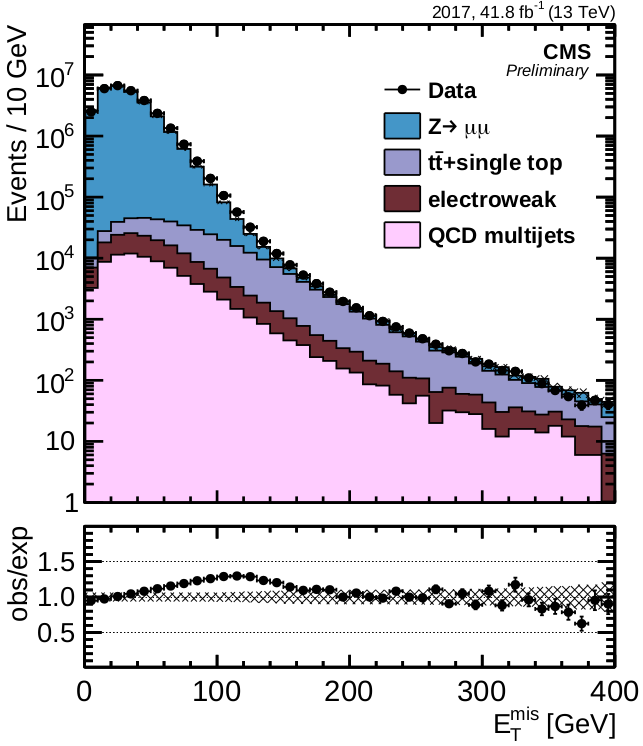
\includegraphics[width=.45\textwidth]{\PhDthesisdir/plots_and_images/from_MET_recoil_Alexei/withoutrecoil.png}}
\hfill
\subcaptionbox{Distribution de \MET\ avec correction.}[.45\textwidth]
{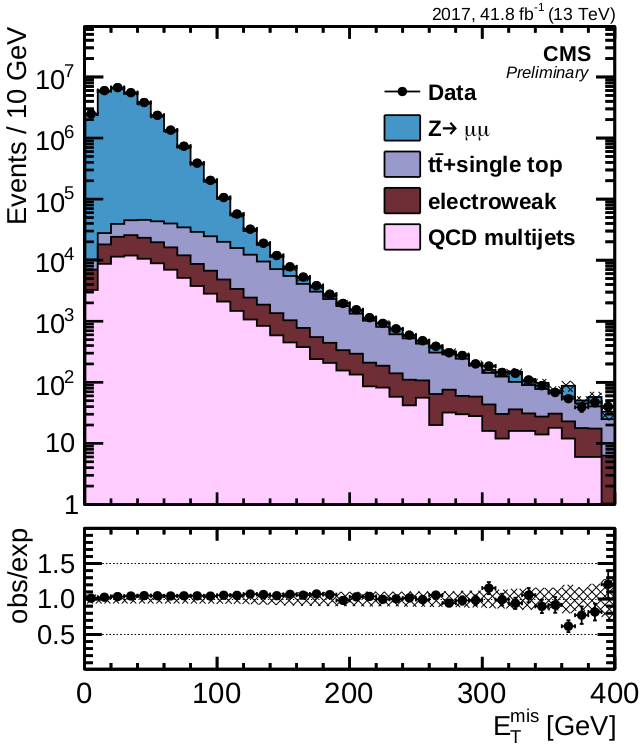
\includegraphics[width=.45\textwidth]{\PhDthesisdir/plots_and_images/from_MET_recoil_Alexei/withrecoil.png}}

\caption[Effet de la correction de recul de \MET.]{Effet de la correction de recul de \MET\ sur une sélection d'événements $\Zboson\to\mu\mu$ en 2017~\cite{MET_recoil_Alexei}.}
\label{fig-MET_recoil_Alexei}
\end{figure}
\subsubsection{Impulsions des particules générées}
\paragraph{Repondération de l'impulsion transverse et de la masse du boson \Zboson\ (\emph{DY \pT-mass reweighting})}
Les impulsions transverses ainsi que la masse invariante des leptons issus de la désintégration du boson \Zboson\ sont corrigées
dans les événements simulés Drell-Yan.
Ces corrections sont déterminées dans une région de contrôle $\Zboson\to\mu\mu$ et n'introduisent pas de modification du nombre total d'événements.
\paragraph{Repondération de l'impulsion transverse du quark~\quarkt\ (\emph{top \pT\ reweighting})}
La modélisation du bruit de fond \ttbar\ est corrigée afin que les données simulées au NLO correspondent au NNLO.
Pour cela, la distribution en \pT\ des quarks~\quarkt\ est pondérée.
La pondération à appliquer à un quark~\quarkt, déterminée par le groupe \quarkt\antiquarkt\Higgs\ s'exprime en fonction de l'impulsion transverse du quark~\quarkt\ en \SI{}{\GeV} selon
\begin{equation}
\omega = \exp(\num{0.088} - \num{8.7e-4}\times\pT + \num{9.2e-7}\times\pT^2)
\mend
\end{equation}
Le poids total à appliquer aux événements \ttbar\ contenant deux quarks~\quarkt\ est alors
\begin{equation}
\omega(\text{total}) = \sqrt{\omega(1) \times \omega(2)}
\mend
\end{equation}